\chapter{Simulation et déploiement}
\label{chap-simulation}

Après l'étude technique de la plateforme, ce chapitre présente la réalisation
du prototype connecté ARGOS et son intégration avec le backend. Il distingue
les éléments effectivement développés, les mécanismes simulés et le protocole
de validation du dispositif physique.

\newcommand{\photoattendue}[1]{%
\begin{figure}[!htbp]
\centering
\fbox{\begin{minipage}[c][5.8cm][c]{0.86\textwidth}
\centering\mbox{}
\end{minipage}}
\caption{#1}
\end{figure}}

\section{Atelier de production}
\subsection{Objectif du prototype}

Le prototype matérialise la boîte noire associée à un conteneur. Il assure
quatre fonctions principales :
\begin{itemize}
    \item acquérir les mesures environnementales et les états de sécurité ;
    \item récupérer une position GNSS et estimer le mouvement et les chocs ;
    \item enregistrer des séquences audio et les transférer vers le stockage
    privé de la plateforme ;
    \item transmettre périodiquement un message de télémétrie au serveur ;
    \item recevoir des modes de fonctionnement et rendre compte de leur
    exécution.
\end{itemize}

La version de firmware fournie dans le projet cible un ESP32. Elle utilise
le Wi-Fi et HTTP pour le développement, un DHT22, un MPU-6050, une carte
microSD, un microphone, un HC-SR04, un détecteur de flamme, un buzzer, une LED
d'état et un récepteur GNSS NEO-6M interprété par TinyGPS++. Le contrat JSON
prévoit aussi la pression et le niveau de batterie. La pression reste fixée à
\SI{1013.25}{\hecto\pascal} tant qu'un BME280 ou BMP280 n'est pas intégré.

\subsection{Déploiement de la plateforme, outils et langages utilisés}

Cette phase relie le prototype à la plateforme ARGOS. Le fichier \code{docker-compose.yml} orchestre PostgreSQL/TimescaleDB, Redis, l'application Flask exécutée par Gunicorn, le worker et Cloudflare Tunnel pour l'accès HTTPS de démonstration. Les volumes Docker préservent les données et les documents privés ; les paramètres sensibles sont fournis par variables d'environnement.

\subsubsection{Outils de réalisation}

Visual Studio Code est utilisé pour l'édition et le débogage du code ; Docker reproduit l'environnement d'exécution ; ChatGPT a servi d'assistant de rédaction et de vérification ; Arduino IDE permet de compiler et téléverser le firmware de l'ESP32 ; \LaTeX{} produit le rapport et Excel facilite les calculs et la préparation des tableaux. La \cref{fig-outils-atelier-argos} regroupe ces outils.

\begin{figure}[!htbp]
\centering
\begin{subfigure}[b]{0.15\textwidth}\centering
  
\includegraphics[height=2.05cm,keepaspectratio]{vscode.png}\caption{VS Code}
\end{subfigure}\hfill
\begin{subfigure}[b]{0.15\textwidth}\centering
  
\includegraphics[height=2.05cm,keepaspectratio]{docker.png}\caption{Docker}
\end{subfigure}\hfill
\begin{subfigure}[b]{0.15\textwidth}\centering
  
\includegraphics[height=2.05cm,keepaspectratio]{images.png}\caption{ChatGPT}
\end{subfigure}\hfill
\begin{subfigure}[b]{0.15\textwidth}\centering
  
\includegraphics[height=2.05cm,keepaspectratio]{arduino.png}\caption{Arduino IDE}
\end{subfigure}\hfill
\begin{subfigure}[b]{0.15\textwidth}\centering
  
\includegraphics[height=2.05cm,keepaspectratio]{latex.png}\caption{\LaTeX}
\end{subfigure}\hfill
\begin{subfigure}[b]{0.15\textwidth}\centering
  
\includegraphics[height=2.05cm,keepaspectratio]{excel.png}\caption{Excel}
\end{subfigure}
\caption{Outils mobilisés pour le prototype et la plateforme ARGOS}
\label{fig-outils-atelier-argos}
\end{figure}

\subsection{Langages utilisés}
Cette section présente les différents langages de programmation mobilisés pour la réalisation de la plateforme ARGOS. Chacun d'eux intervient à un niveau spécifique du système, qu'il s'agisse du traitement des données côté serveur ou de la présentation et de l'interactivité de l'interface utilisateur. Cette présentation permet de situer le rôle de chaque technologie dans l'architecture globale du projet.
\begin{itemize}
    \item \textbf{Python} : il nous permet d'implémenter les services Flask, les traitements métier, l'accès aux données et le simulateur IoT.
    \item \textbf{HTML/CSS} : ils nous permettent de mieux structurer les pages web et de définir leur présentation responsive pour les utilisateurs de la plateforme.
    \item \textbf{JavaScript} : il nous permet d'apporter l'interactivité de l'interface, les requêtes vers l'API, les cartes et l'actualisation des données.
\end{itemize}

\subsection{Architecture fonctionnelle du prototype}

\begin{figure}[!htbp]
\centering
\resizebox{0.98\linewidth}{!}{%
\begin{tikzpicture}[font=\sffamily\small,
 block/.style={draw=argosnavy,rounded corners=2pt,align=center,minimum width=3.5cm,minimum height=1.15cm,fill=argospale},
 core/.style={block,minimum width=4.4cm,minimum height=1.65cm,fill=argoslight,line width=1.1pt},
 flow/.style={-{Stealth[length=2.5mm]},draw=argosmid,line width=.9pt},
 bidir/.style={{Stealth[length=2.5mm]}-{Stealth[length=2.5mm]},draw=argosmid,line width=.9pt}]
\node[core] (esp) at (0,0) {ESP32\\acquisition, fusion et file locale};
\node[block] (env) at (-7,3) {DHT22 + BME280\\température, humidité, pression};
\node[block] (motion) at (-7,1) {MPU-6050\\accélération, choc};
\node[block] (security) at (-7,-1) {flamme + HC-SR04\\lumière, porte, distance};
\node[block] (audio) at (-7,-3) {microphone\\niveau sonore et WAV};
\node[block] (gnss) at (0,3.4) {NEO-6M\\position, vitesse, cap};
\node[block] (sd) at (0,-3.4) {microSD\\télémétries et audio en attente};
\node[block] (network) at (7,2) {sélecteur multiréseau\\Wi-Fi / LTE-M / NB-IoT / LoRaWAN};
\node[block] (sat) at (7,0) {satellite IoT\\secours hors couverture};
\node[block] (argos) at (7,-2.4) {Plateforme ARGOS\\HTTP REST + MQTT/TLS};
\draw[flow] (env.east) -- (esp.west);
\draw[flow] (motion.east) -- (esp.west);
\draw[flow] (security.east) -- (esp.west);
\draw[flow] (audio.east) -- (esp.west);
\draw[bidir] (gnss.south) -- (esp.north);
\draw[bidir] (sd.north) -- (esp.south);
\draw[bidir] (esp.east) -- (network.west);
\draw[bidir] (esp.east) -- (sat.west);
\draw[bidir] (network.south east) -- (argos.north east);
\draw[bidir] (sat.south east) -- (argos.north);
\end{tikzpicture}%
}

\caption{Architecture fonctionnelle du prototype ARGOS}
\label{fig-argos-prototype-fonctionnel}
\end{figure}
\tablesourcepromoteurs

La \cref{fig-argos-prototype-fonctionnel} place l'ESP32 au centre du
prototype. Les capteurs fournissent les mesures à l'unité de traitement. Le
GNSS et le modem échangent leurs données par UART ; le MPU-6050 utilise I²C et
la carte microSD utilise SPI. Après agrégation, les données sont sérialisées en
JSON puis transmises vers la plateforme ARGOS. Les enregistrements audio sont
envoyés séparément sous forme de fichiers multiparties.

Les flèches du schéma sont uniquement utilisées lorsqu'un sens de circulation
est défini : acquisition d'une mesure vers l'ESP32, commande d'une sortie
depuis l'ESP32 ou transmission réseau vers la plateforme.

\subsection{Composition matérielle}

Cette section présente l'architecture matérielle de notre dispositif. Pour garantir les performances, la fiabilité et l'efficacité de notre système, chaque composant a été rigoureusement sélectionné. Les points suivants détaillent les différents modules, cartes et éléments électroniques qui constituent le cœur opérationnel de notre ensemble.

\subsubsection{Unité centrale ESP32}

L'ESP32 exécute le firmware, lit les entrées, pilote les sorties, dialogue
avec le GNSS et communique avec le serveur. Le port série de diagnostic est
initialisé à 115\,200 bauds et le NEO-6M à 9\,600 bauds. La mémoire NVS conserve
le \code{deviceUid}, le \code{blackBoxId}, l'affectation au conteneur et la clé
technique après l'enrôlement.

\begin{figure}[!htbp]
\centering
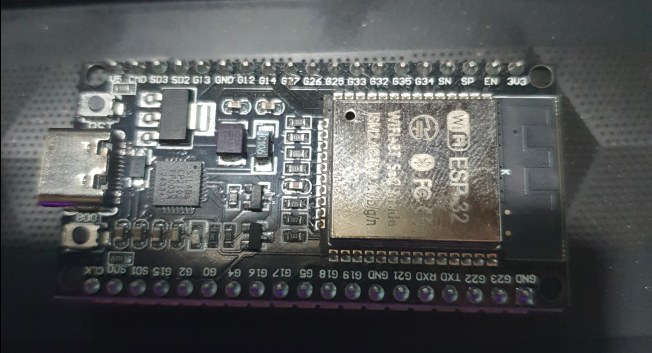
\includegraphics[width=0.56\textwidth]{figures/eespp.png}
\caption{Carte ESP32 utilisée pour le prototype ARGOS}
\label{fig-argos-esp32}
\end{figure}
\tablesourcepromoteurs

\subsubsection{Capteur de température et d'humidité}

Le firmware déclare un AM2302/DHT22 raccordé au GPIO~4. Il fournit les valeurs
\code{temperature} et \code{humidity} du message de télémétrie. Toute
conclusion sur sa précision doit être fondée sur un étalonnage ou sur la fiche
technique exacte du composant monté.

\begin{figure}[!htbp]
\centering
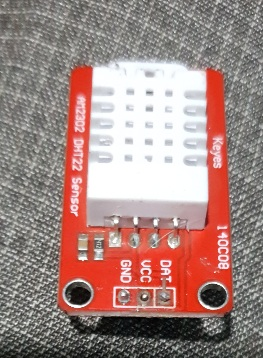
\includegraphics[width=0.26\textwidth]{figures/dht22.jpg}
\caption{Capteur de température et d'humidité}
\label{fig-argos-am2302}
\end{figure}
\tablesourcepromoteurs

\subsubsection{Pression, mouvement et détection de choc}

Le MPU-6050 est raccordé au bus I²C, SDA sur GPIO~8 et SCL sur GPIO~9. Le choc
instantané est exprimé en multiples de l'accélération de la pesanteur :
\begin{equation}
 a_m=\sqrt{a_x^2+a_y^2+a_z^2},\qquad
 choc=\frac{|a_m-g|}{g},\quad g=\SI{9.80665}{\metre\per\second\squared}.
\end{equation}
Une calibration des biais, un filtrage et la conservation du maximum sur une
courte fenêtre sont nécessaires pour limiter les faux positifs. La vitesse de
référence provient du GNSS. Une intégration de l'accélération horizontale du
MPU peut seulement combler une brève perte GNSS, car la dérive rend une vitesse
calculée uniquement par centrale inertielle rapidement inexploitable.

La pression atmosphérique nécessite l'ajout d'un BME280 ou BMP280 sur le même
bus I²C. Jusqu'à cette intégration, la valeur envoyée par le firmware est une
constante de compatibilité et non une observation du milieu.

\begin{figure}[!htbp]
\centering
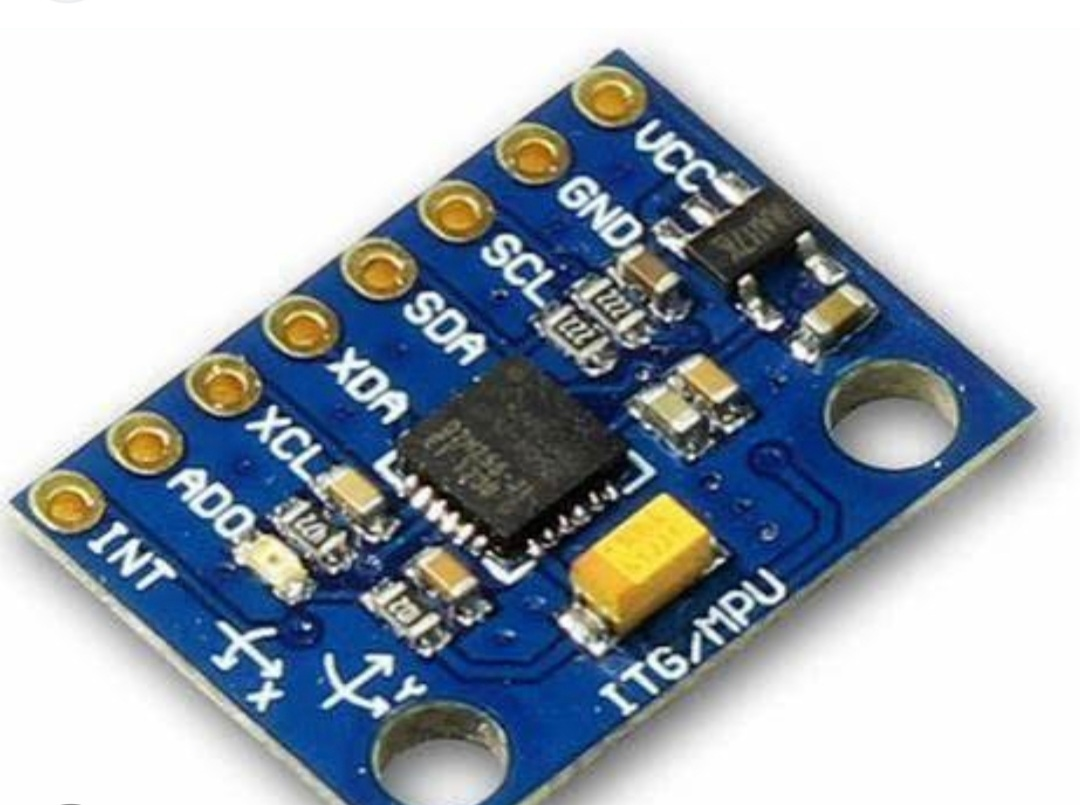
\includegraphics[width=0.26\textwidth]{figures/sda.jpg}
\caption{Pression, mouvement et détection de choc}
\label{fig-argos-BME}
\end{figure}
\tablesourcepromoteurs

\subsubsection{Détection de flamme et acquisition audio}

Le détecteur de flamme est raccordé au GPIO~21 et le microphone analogique au
GPIO~5. Le niveau sonore est inclus dans la télémétrie. Pour produire un son
lisible, le firmware doit échantillonner le signal, construire un fichier WAV,
le conserver temporairement sur la microSD puis l'envoyer à
\code{/api/iot/audio}. Le backend limite actuellement un fichier à 25~Mio,
calcule son empreinte SHA-256 et le place dans le stockage privé. Un découpage
en segments de 5 à 30 secondes fournit un quasi-direct compatible avec les
coupures réseau ; ce mécanisme ne constitue pas un flux audio continu.

\begin{figure}[!htbp]
\centering
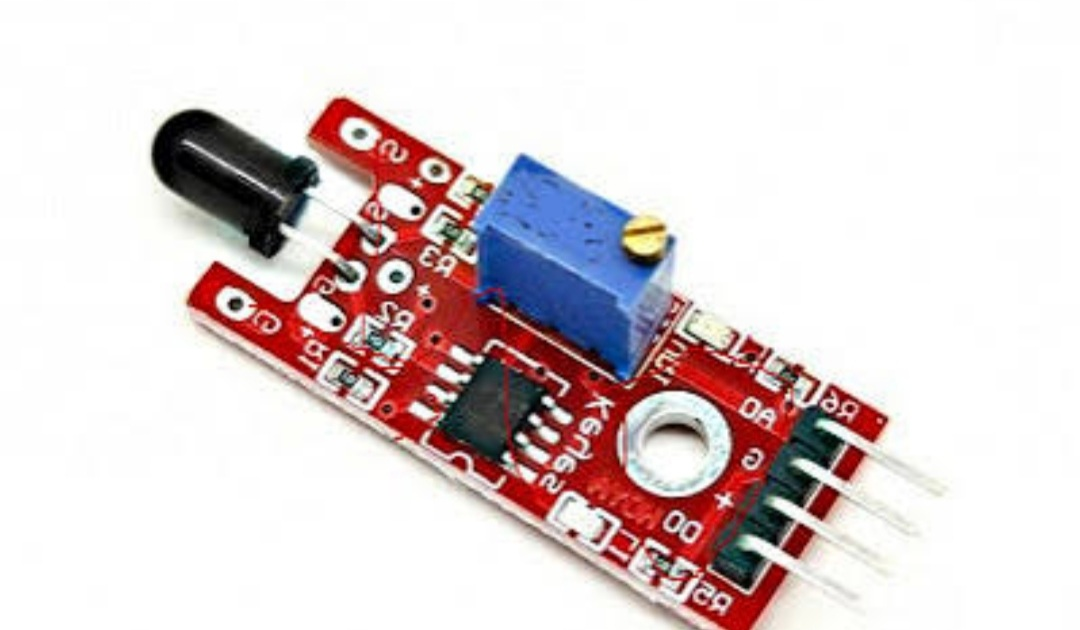
\includegraphics[width=0.26\textwidth]{figures/fl.jpg}
\caption{Module de Détection de flamme}
\label{fig-argos-flamme}
\end{figure}
\tablesourcepromoteurs

\subsubsection{Module de géolocalisation}

Le NEO-6M communique avec l'ESP32 par UART : TX du GPS vers GPIO~17 et RX du
GPS vers GPIO~18. TinyGPS++ interprète les trames et fournit latitude,
longitude, vitesse et cap. Les coordonnées alimentent directement les tables
de positions et le marqueur Leaflet de la boîte noire. En l'absence de position
valide, la donnée doit être qualifiée comme indisponible et la dernière
position valide peut être affichée avec son horodatage.

\begin{figure}[!htbp]
\centering
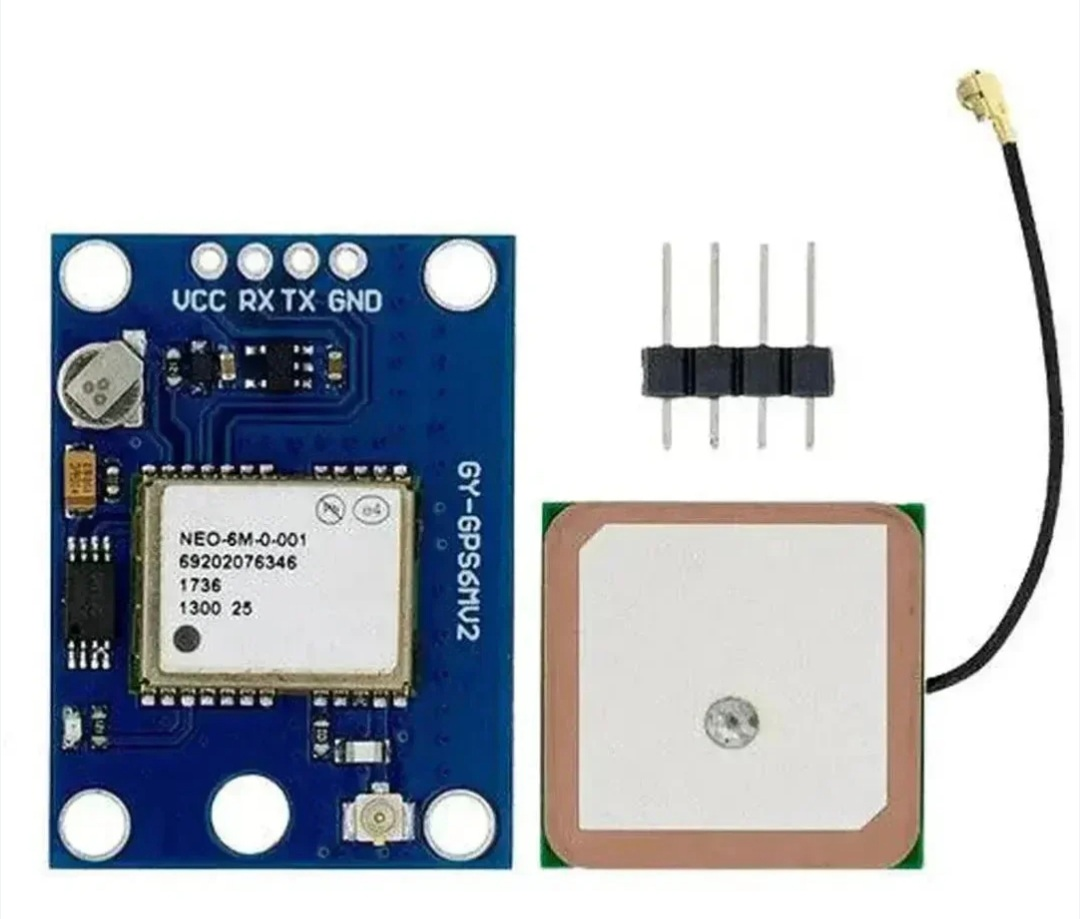
\includegraphics[width=0.26\textwidth]{figures/asp.jpg}
\caption{Module GPS du prototype ARGOS}
\label{fig-argos-gps}
\end{figure}
\tablesourcepromoteurs

\subsubsection{Alimentation et signalisation}

La LED bleue est raccordée au GPIO~1 et le buzzer actif au GPIO~10. La LED
indique que le Wi-Fi, l'identité du boîtier, son affectation, le MPU-6050 et la
carte SD sont opérationnels. Le choix définitif de la batterie, du régulateur, des
protections et du boîtier doit être documenté à partir du montage réellement
assemblé. L'autonomie ne doit être annoncée qu'après mesure du courant dans
les différents modes.

\begin{figure}[!htbp]
\centering
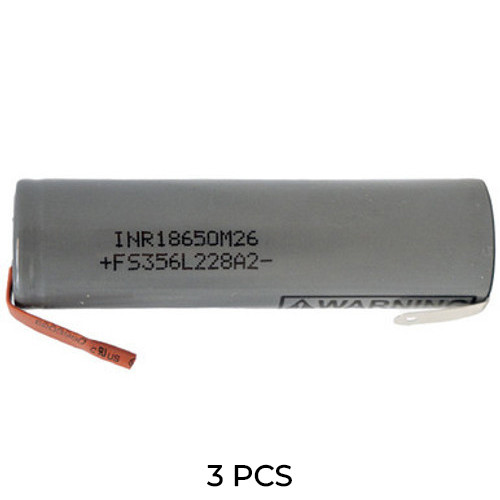
\includegraphics[width=0.26\textwidth]{figures/pile.jpg}
\caption{Alimentation}
\label{fig-argos-alimentation}
\end{figure}
\tablesourcepromoteurs


\section{Processus de réalisation}
\subsection{Connectivité terrestre et maritime}

Le Wi-Fi demeure le canal du prototype de laboratoire et de la configuration
locale. Pour l'exploitation mobile internationale, l'architecture retient une
stratégie multiréseau :
\begin{itemize}
    \item LTE-M ou NB-IoT avec profil eSIM et itinérance multi-opérateurs pour
    les zones terrestres et portuaires couvertes ;
    \item LoRaWAN pour les ports, entrepôts et corridors équipés de passerelles,
    avec itinérance entre opérateurs lorsqu'elle est contractuellement disponible ;
    \item satellite IoT à faible débit comme secours en mer et dans les zones
    isolées dépourvues de couverture terrestre.
\end{itemize}

LoRaWAN est une technologie longue portée et basse consommation, mais sa
couverture internationale dépend d'infrastructures de passerelles et de
réseaux interconnectés. Le satellite complète donc LoRaWAN et les réseaux
cellulaires ; il n'est sollicité que pour les messages prioritaires afin de
maîtriser l'énergie, le débit et le coût. Le firmware place les messages non
confirmés dans une file sur microSD, conserve une séquence croissante et les
retransmet après le rétablissement d'un canal.

\begin{figure}[!htbp]
\centering
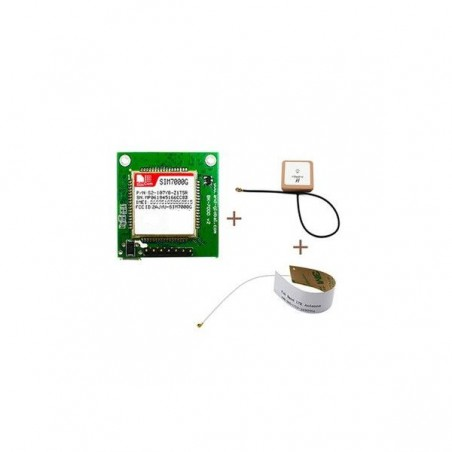
\includegraphics[width=0.56\textwidth]{figures/sim.jpg}
\caption{Sim 800l LTE-4G}
\label{fig-argos-sim}
\end{figure}
\tablesourcepromoteurs


\subsection{Schéma de raccordement}

Le schéma de raccordement formalise l'architecture matérielle et les interconnexions physiques du prototype ARGOS, articulé autour de la carte microcontrôlée principale et de ses périphériques capteurs. Cette vue d'ensemble est essentielle pour garantir la conformité du montage électronique, la fiabilité des transmissions de données et l'alimentation stable des composants embarqués en condition réelle.

\begin{figure}[!htbp]
\centering
\resizebox{0.85\textwidth}{!}{%
  \resizebox{0.98\linewidth}{!}{%
\begin{tikzpicture}[font=\sffamily\scriptsize,
 module/.style={draw=argosnavy,rounded corners=2pt,align=left,minimum width=4cm,minimum height=.9cm,fill=white},
 mcu/.style={draw=argosnavy,rounded corners=2pt,align=center,minimum width=4.2cm,minimum height=7cm,fill=argoslight,line width=1.1pt},
 wire/.style={draw=argosmid,line width=.8pt}]
\node[mcu] (mcu) at (0,0) {\textbf{ESP32}\\[3pt]
GPIO 1 : LED\\\\GPIO 4 : DHT22 (ou autre)\\GPIO 5 : SCL (I²C)\\
GPIO 13 : buzzer\\GPIO 14 : MOSI (SD)\\GPIO 15 : RX (GPS)\\GPIO 16 : ECHO (HC-SR04)\\
GPIO 17 : flamme\\GPIO 18 : TRIG (HC-SR04)\\GPIO 21 : SDA (I²C)\\GPIO 22 : microphone\\
GPIO 26 : SCK (SD)\\GPIO 27 : MISO (SD)};
\node[module] (dht) at (-7,3.3) {DHT22 : DATA $\rightarrow$ GPIO 4};
\node[module] (analog) at (-7,1.9) {Microphone : GPIO 22};
\node[module] (ultra) at (-7,.5) {HC-SR04 : TRIG 18, ECHO 16\footnotemark};
\node[module] (i2c) at (-7,-.9) {MPU-6050 + BME280 : SDA 21, SCL 5};
\node[module] (alarm) at (-7,-2.3) {LED / Buzzer / Flamme : GPIO 1 / 13 / 17};
\node[module] (sd) at (7,3.3) {microSD SPI : MOSI 14, SCK 26, MISO 27};
\node[module] (modem) at (7,1.4) {Modem LTE-M/NB-IoT ou LoRaWAN};
\node[module] (gnss) at (7,-.5) {NEO-6M UART : TX $\rightarrow$ 2, RX $\leftarrow$ 15};
\node[module] (sat) at (7,-2.4) {Modem satellite IoT\\UART/SPI selon module};
\foreach \n in {dht,analog,ultra,i2c,alarm} \draw[wire] (\n.east) -- (mcu.west |- \n.east);
\foreach \n in {sd,modem,gnss,sat} \draw[wire] (mcu.east |- \n.west) -- (\n.west);
\end{tikzpicture}%
}
\footnotetext{La sortie ECHO 5 V du HC-SR04 doit être abaissée à 3,3 V par pont diviseur ou convertisseur de niveau.}%
}
\caption{Schéma de raccordement logique du prototype ARGOS}
\label{fig-argos-cablage}
\end{figure}
\tablesourcepromoteurs

Le dispositif repose principalement sur le module ESP32-S3, qui centralise l'acquisition des données métrologiques et géographiques. Les bus de communication numérique (I2C et SPI) interconnectent les capteurs de position, d'inertie et environnementaux, tandis que les interfaces spécifiques gèrent le module de téléphonie mobile et les capteurs analogiques. Cette disposition modulaire assure une maintenance aisée du prototype tout en garantissant l'intégrité des signaux électriques face aux perturbations électromagnétiques rencontrées sur le terrain.

\par Le schéma de la \cref{fig-argos-cablage} présente les raccordements définis
dans le firmware. Les traits orientés représentent les signaux d'entrée ou de
sortie. Les liaisons d'alimentation sont séparées des données. Avant la mise
sous tension, il est indispensable de vérifier la tension admissible de
chaque module, de partager une masse commune et d'empêcher qu'une entrée
analogique reçoive une tension supérieure à la limite de l'ESP32.

\begin{figure}[!htbp]
\centering
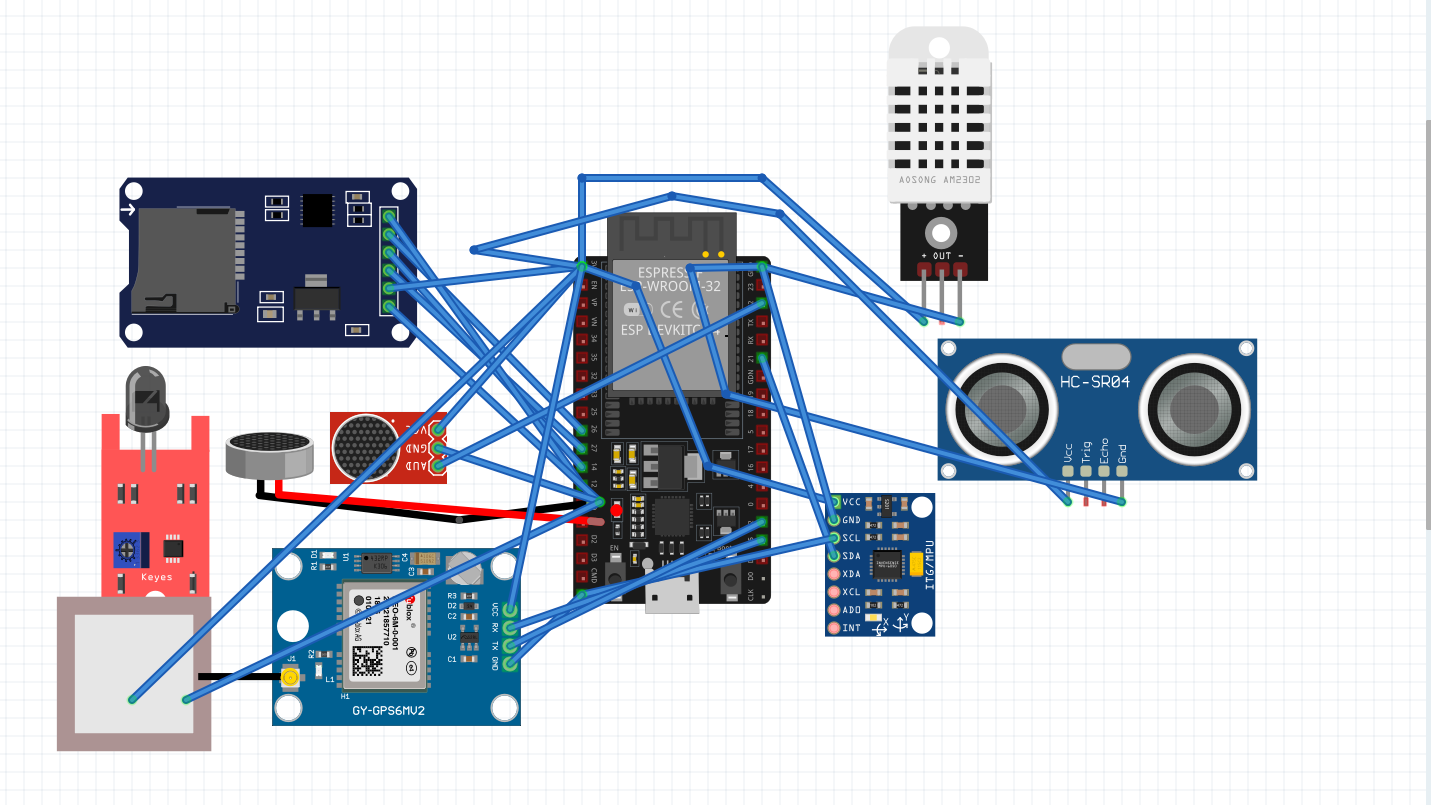
\includegraphics[width=0.86\textwidth]{figures/platine_de.png}
\caption{Vue générale du câblage réel}
\label{fig-cablages-jumpeur}
\end{figure}
\tablesourcepromoteurs

\begin{figure}[!htbp]
\centering
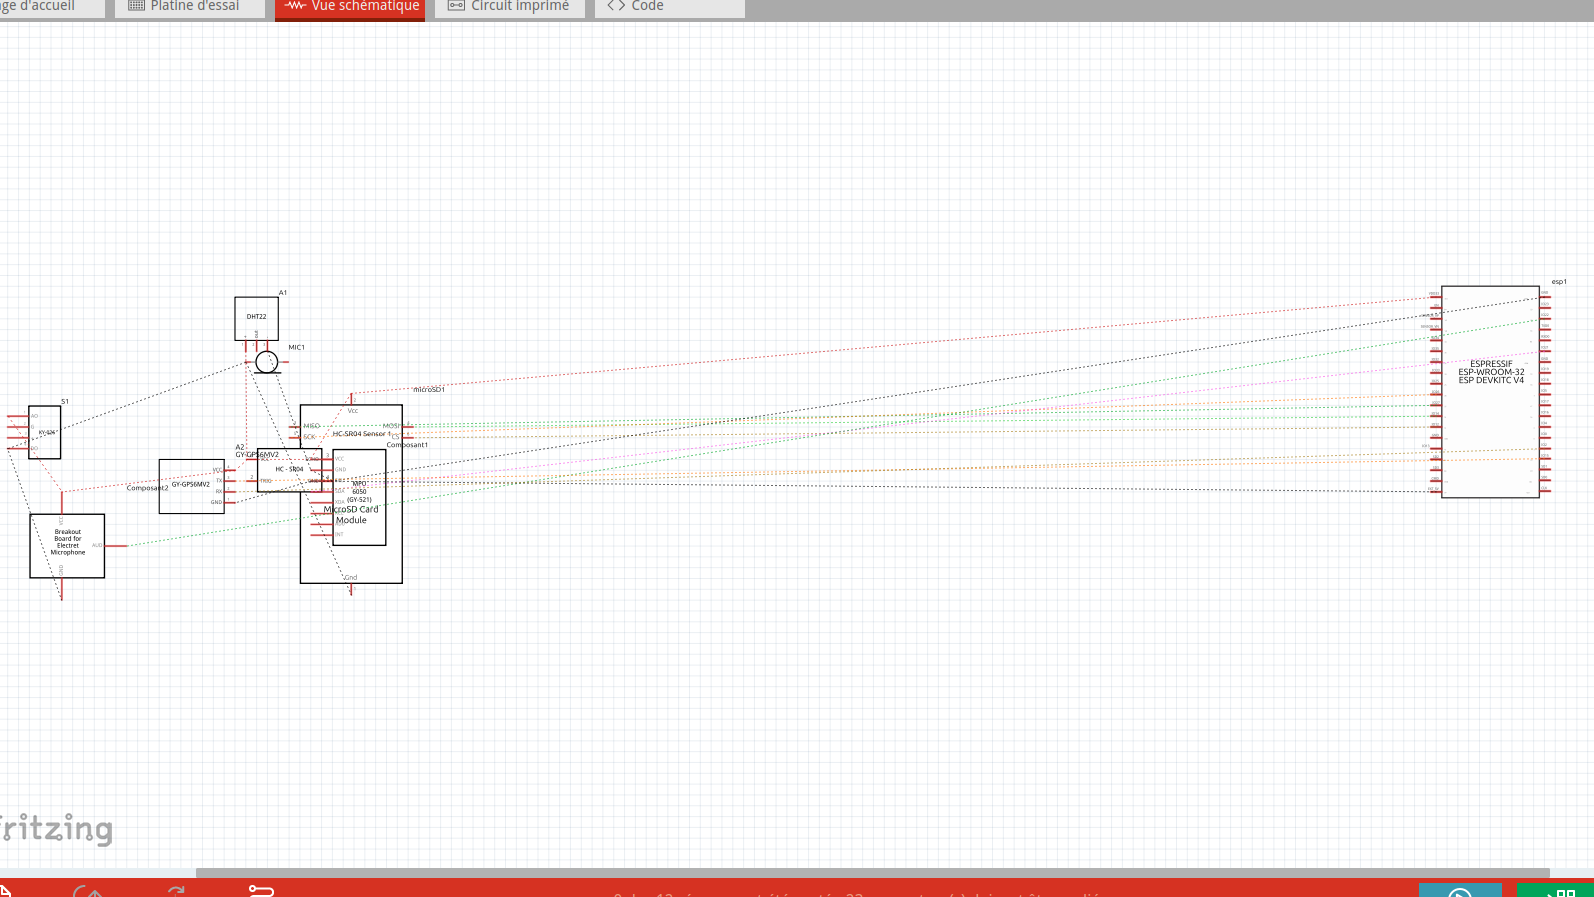
\includegraphics[width=0.86\textwidth]{figures/shemat.png}
\caption{Vue générale du câblage imprimé}
\label{fig-cablages-imprimer}
\end{figure}
\tablesourcepromoteurs


\subsection{Organisation du firmware}

Cette section décrit le fonctionnement interne du micrologiciel embarqué sur l'ESP32, depuis son initialisation jusqu'à la construction et l'envoi des messages de télémétrie. Elle détaille les principales étapes exécutées par le programme, notamment la mise en route des différents modules, l'enrôlement du dispositif et la collecte des mesures issues des capteurs. Cette présentation permet de comprendre comment les données physiques acquises par le prototype sont transformées en informations exploitables par la plateforme.

\subsubsection{Initialisation}

Au démarrage, le programme initialise les interfaces série, I²C et SPI, les
broches, le DHT22, le MPU-6050, la microSD, le GNSS et le canal réseau. Lors du premier usage, la fonction
\code{enrollDevice()} envoie le \code{deviceUid} et le jeton d'enrôlement à
\code{/api/iot/enroll}. Si la demande est acceptée, le serveur retourne une
clé permanente utilisée pour les échanges suivants.

\subsubsection{Acquisition et construction du message}

La fonction \code{sendTelemetry()} lit les capteurs et construit un document
JSON contenant :
\begin{itemize}
    \item un identifiant de message, l'identité du dispositif et une séquence ;
    \item la date, le type du message et la version implicite du protocole ;
    \item la position, la précision, la vitesse et le cap ;
    \item les mesures de température, humidité, choc, pression, niveau sonore,
    distance et accélérations triaxiales ;
    \item les indicateurs de flamme, porte, batterie et modes actifs.
\end{itemize}

Le message est envoyé à \code{/api/iot/telemetry} avec la clé du dispositif
dans l'en-tête \code{X-Device-Key}. Le serveur répond avec un code HTTP et un
résultat JSON affichés sur le port série.

\subsubsection{Commandes et audio}

Le backend expose la consultation de l'état, les commandes et la réception
d'un fichier audio authentifié. Il reconnaît les commandes
de sécurité, écoute, enregistrement, détection de flamme, demande de position,
demande d'état et alerte locale. Le cycle complet prévoit un accusé
\code{ACKNOWLEDGED}, puis un résultat final tel que \code{SUCCEEDED} ou
\code{FAILED}.

\subsection{Protocole d'intégration avec la plateforme}

L'intégration suit le cycle ci-dessous :
\begin{enumerate}
    \item création préalable d'une boîte noire dans ARGOS ;
    \item provisionnement du dispositif par un superadministrateur ou un
    propriétaire autorisé ;
    \item configuration du \code{deviceUid} et du jeton temporaire ;
    \item enrôlement du prototype et réception de la clé permanente ;
    \item transmission périodique de la télémétrie avec
    \code{blackBoxId}, \code{containerId}, UUID et séquence croissante ;
    \item transfert séparé des segments audio authentifiés ;
    \item validation, normalisation et stockage par le backend ;
    \item génération éventuelle d'un événement et d'une notification ;
    \item publication des commandes et retour des accusés de réception.
\end{enumerate}

En production, les échanges doivent utiliser TLS. La clé permanente ne doit
pas être écrite dans les journaux et doit être conservée dans une zone
persistante protégée. Un dispositif compromis peut être révoqué côté serveur.

\subsection{Présentation du prototype assemblé}

Les vues du montage documentent son organisation interne, son enveloppe et
son intégration au support de transport.

\begin{figure}[!htbp]
\centering
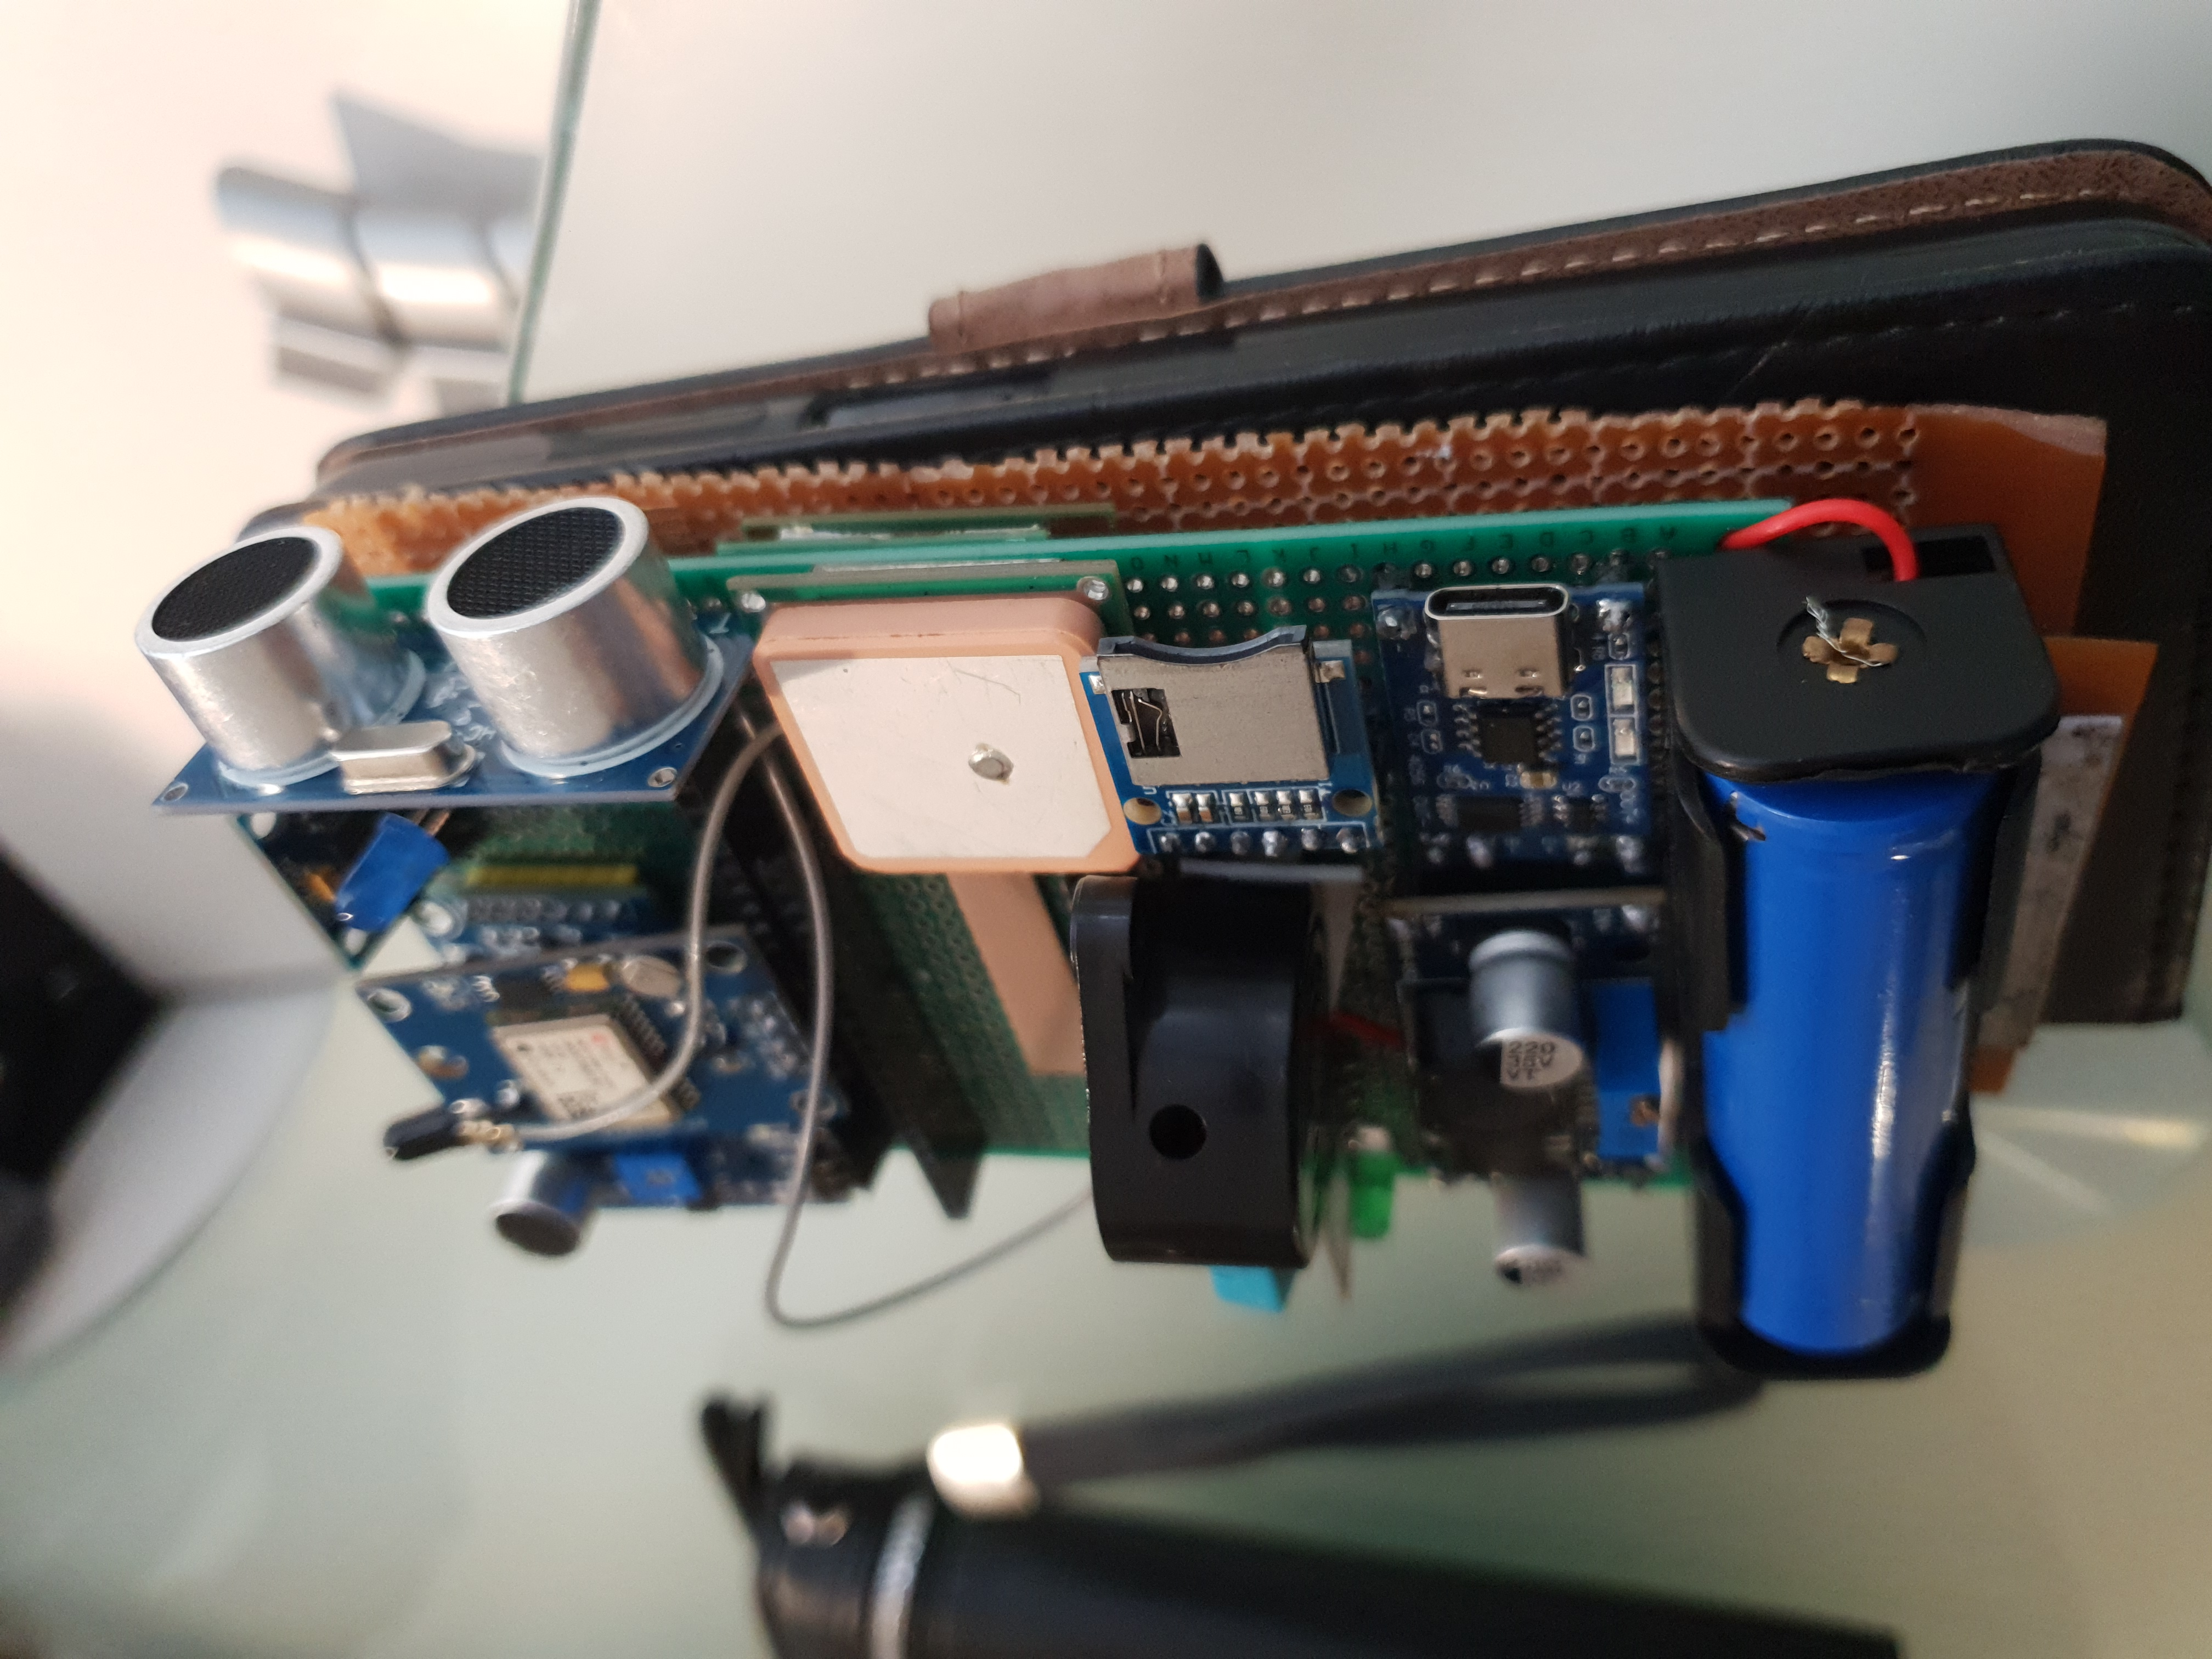
\includegraphics[width=0.86\textwidth, angle=180]{figures/argosint.png}
\caption{Vue interne du prototype ARGOS assemblé}
\label{fig-prototype-argos-interieur}
\end{figure}
\tablesourcepromoteurs

\begin{figure}[!htbp]
\centering
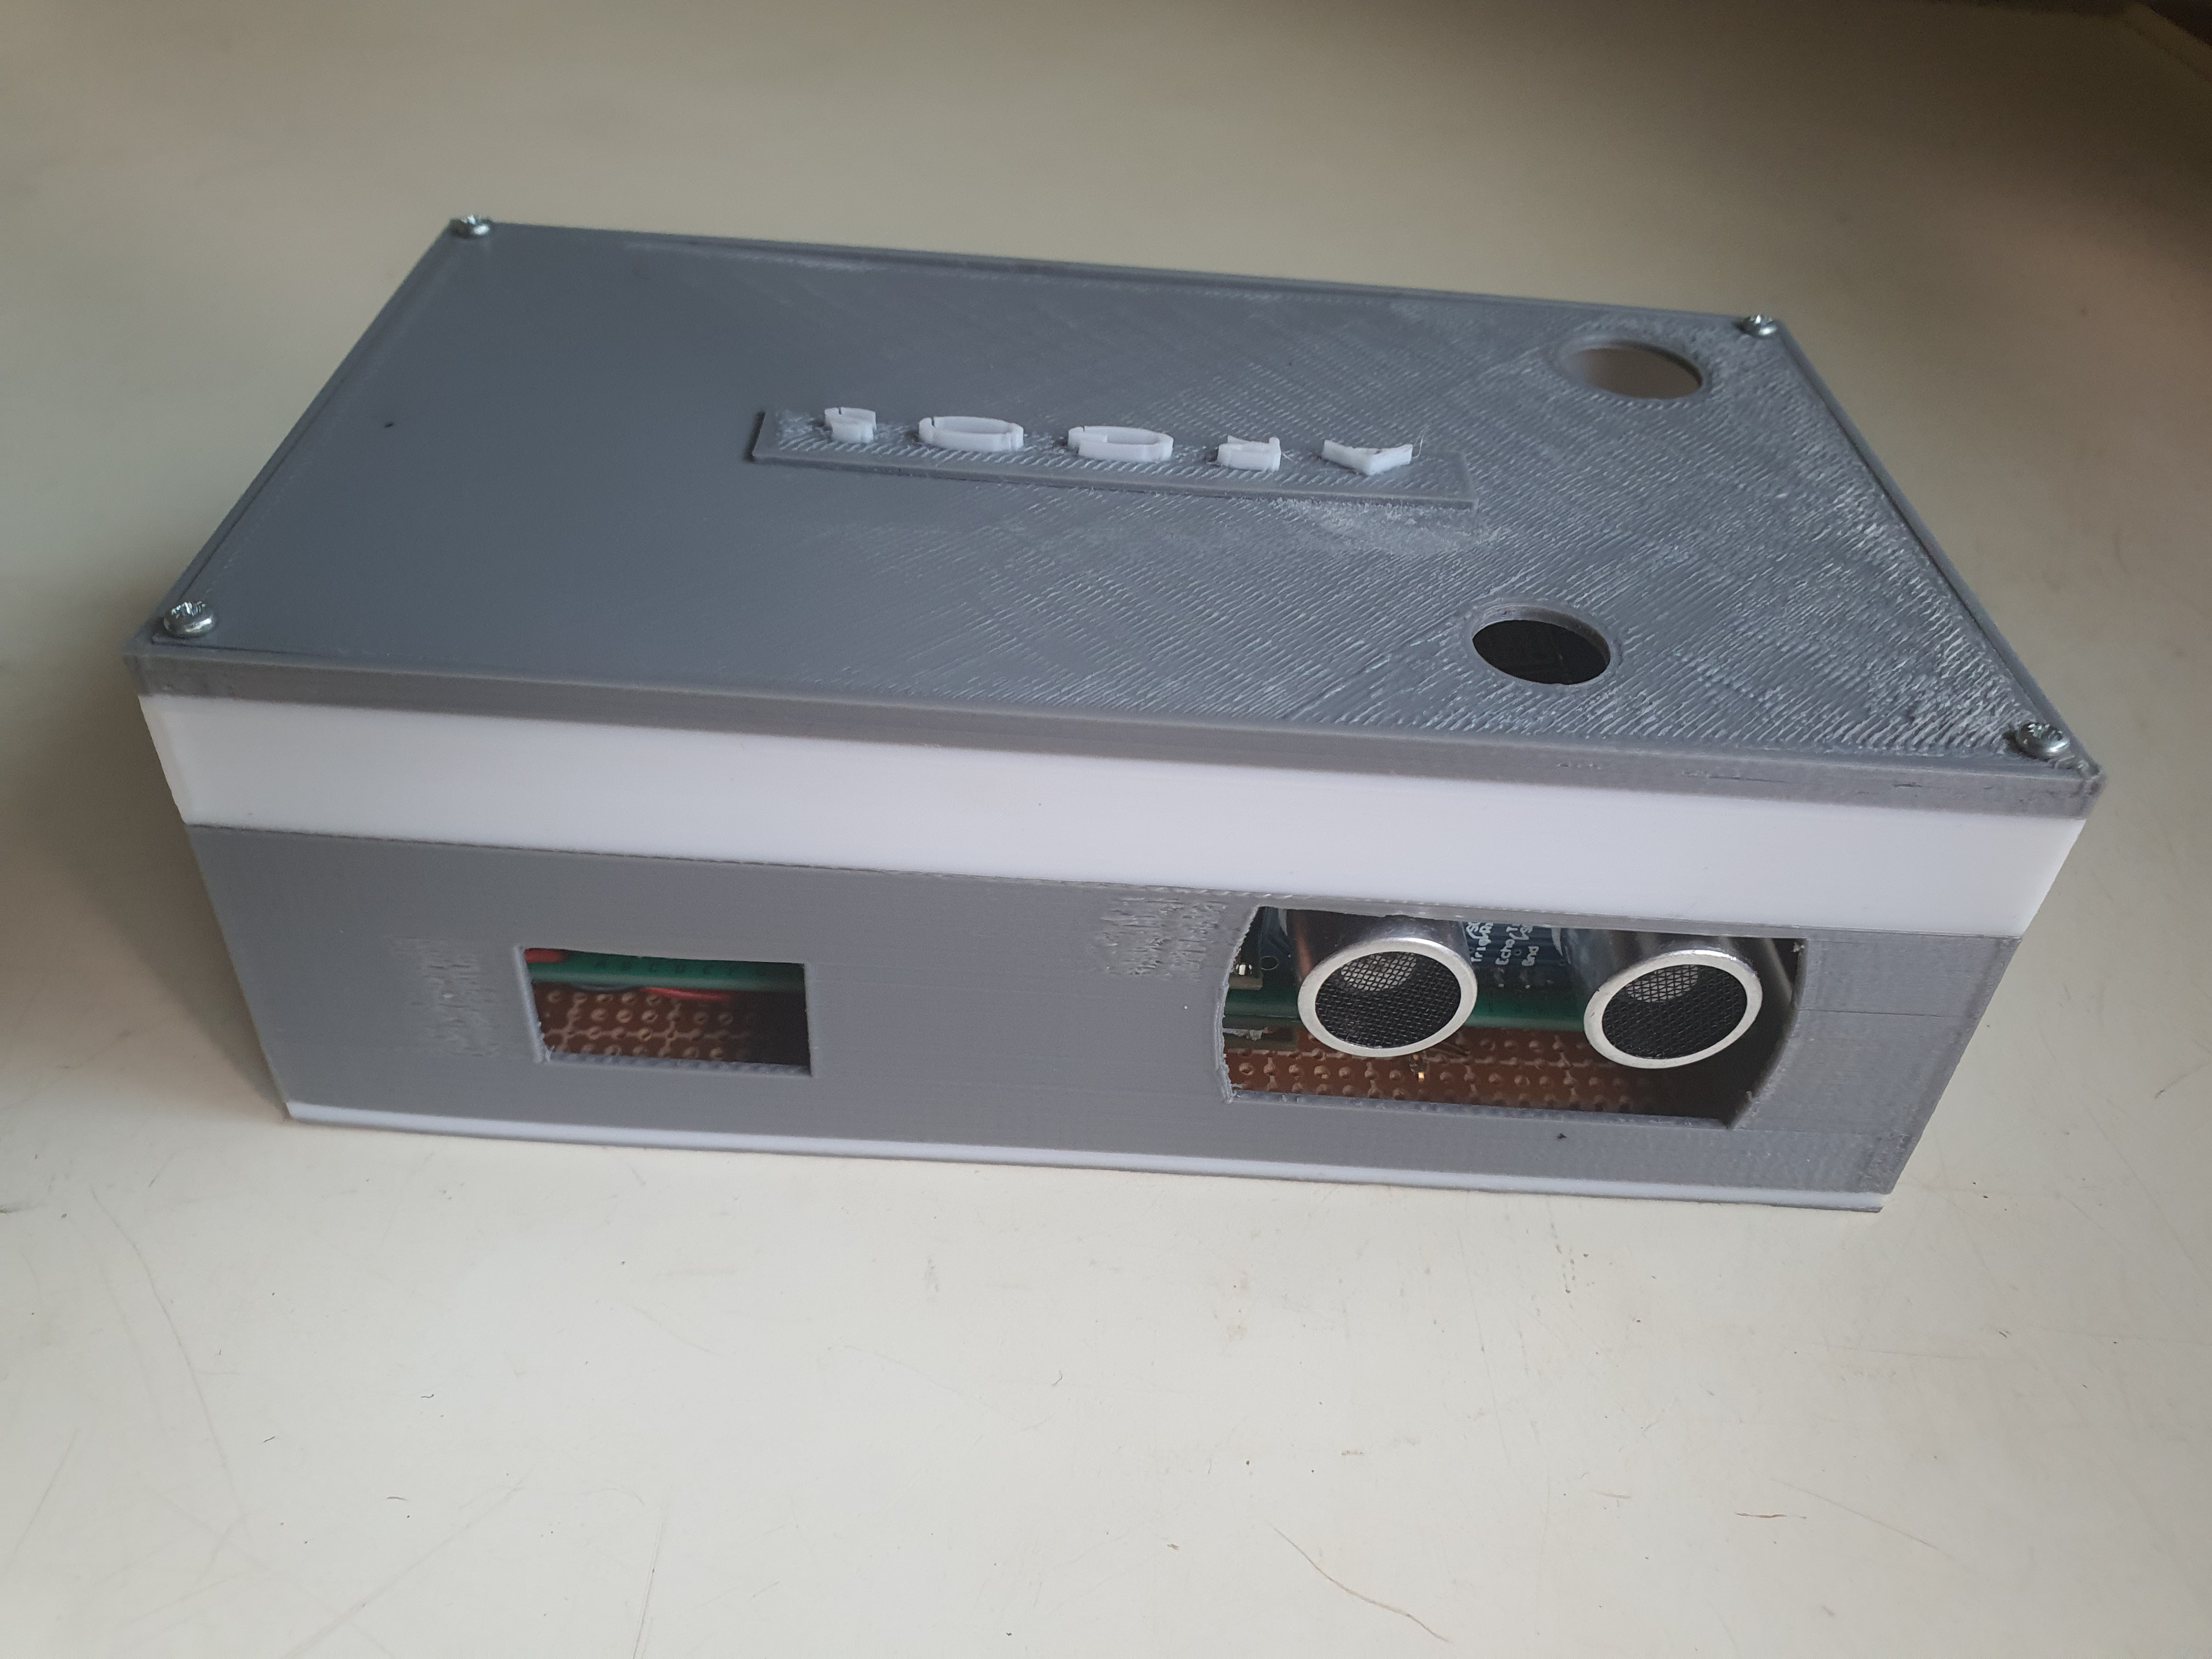
\includegraphics[width=0.86\textwidth]{figures/argosface.png}
\caption{Aspect extérieur du prototype ARGOS}
\label{fig-prototype-argos-exterieur}
\end{figure}
\tablesourcepromoteurs

\subsection{Interfaces de démonstration}

Les interfaces web permettent de vérifier visuellement le résultat des
traitements : authentification, affichage des conteneurs, carte, alertes,
boîtes noires et statistiques.

\begin{figure}[!htbp]
\centering
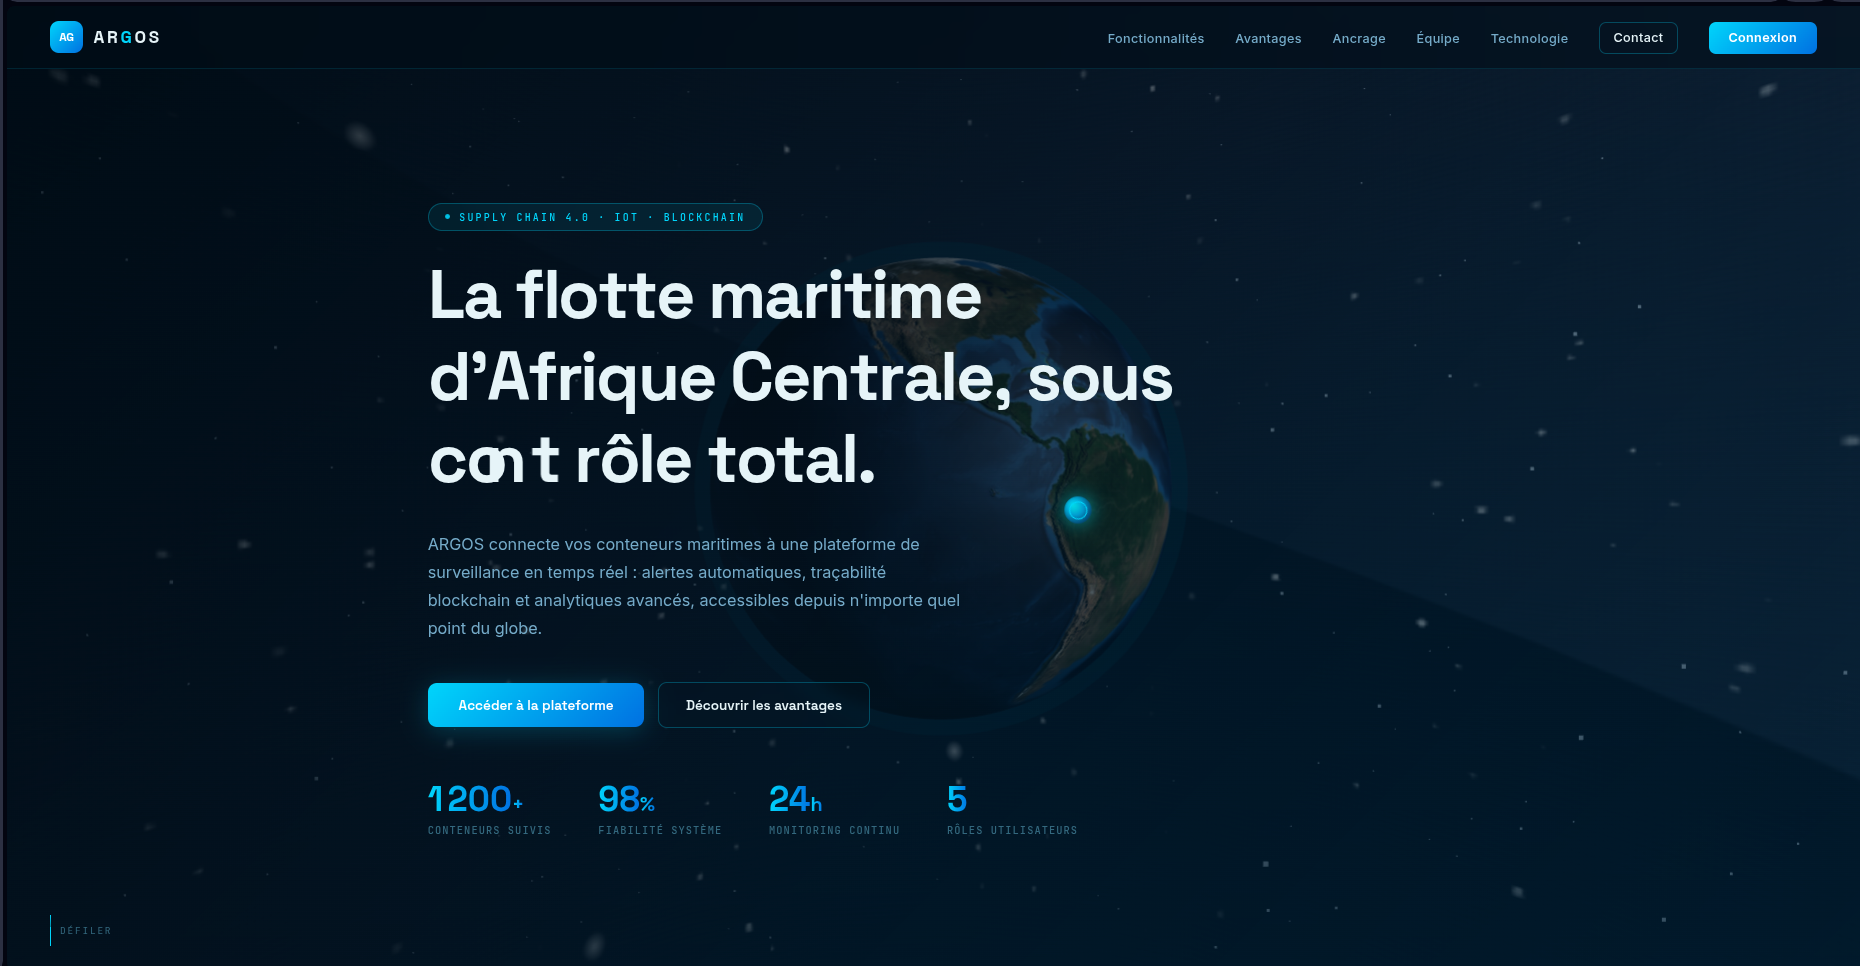
\includegraphics[width=0.66\textwidth]{figures/vitrine.png}
\caption{Page publique de présentation d'ARGOS}
\label{fig-vitrine-argos}
\end{figure}
\tablesourcepromoteurs

\begin{figure}[!htbp]
\centering
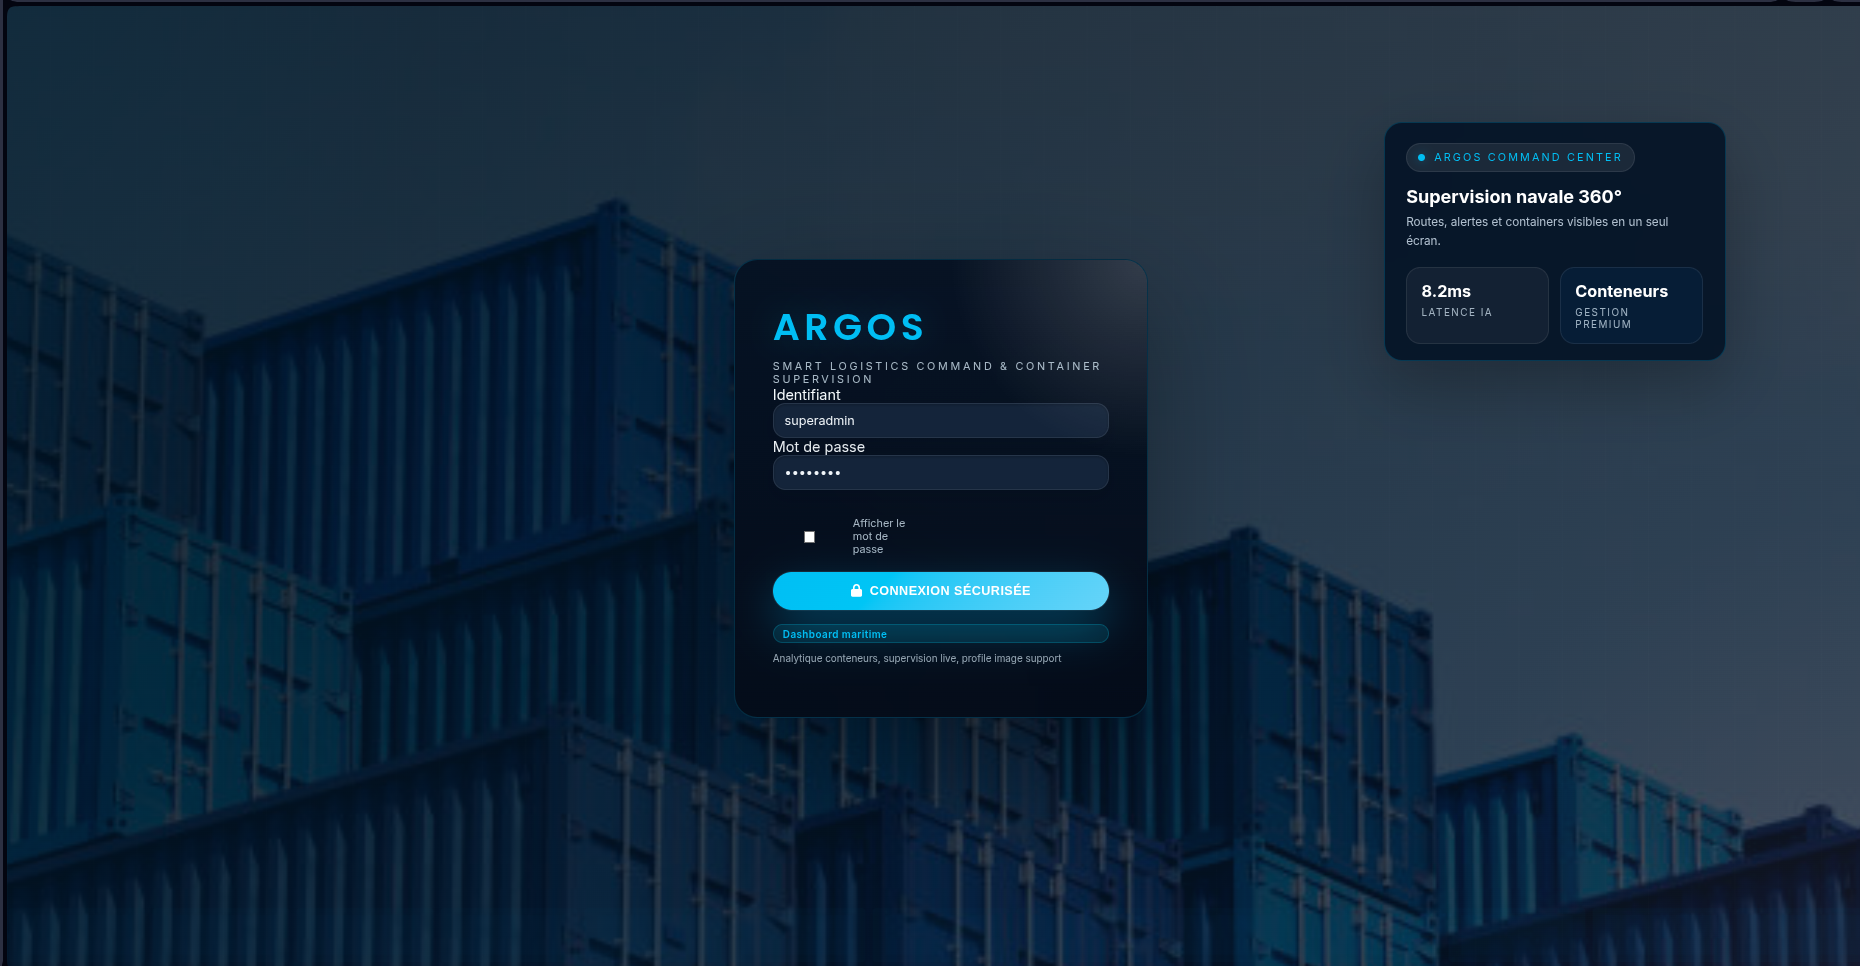
\includegraphics[width=0.66\textwidth]{figures/log.png}
\caption{Interface d'authentification d'ARGOS}
\label{fig-auth-argos}
\end{figure}
\tablesourcepromoteurs

\begin{figure}[!htbp]
\centering
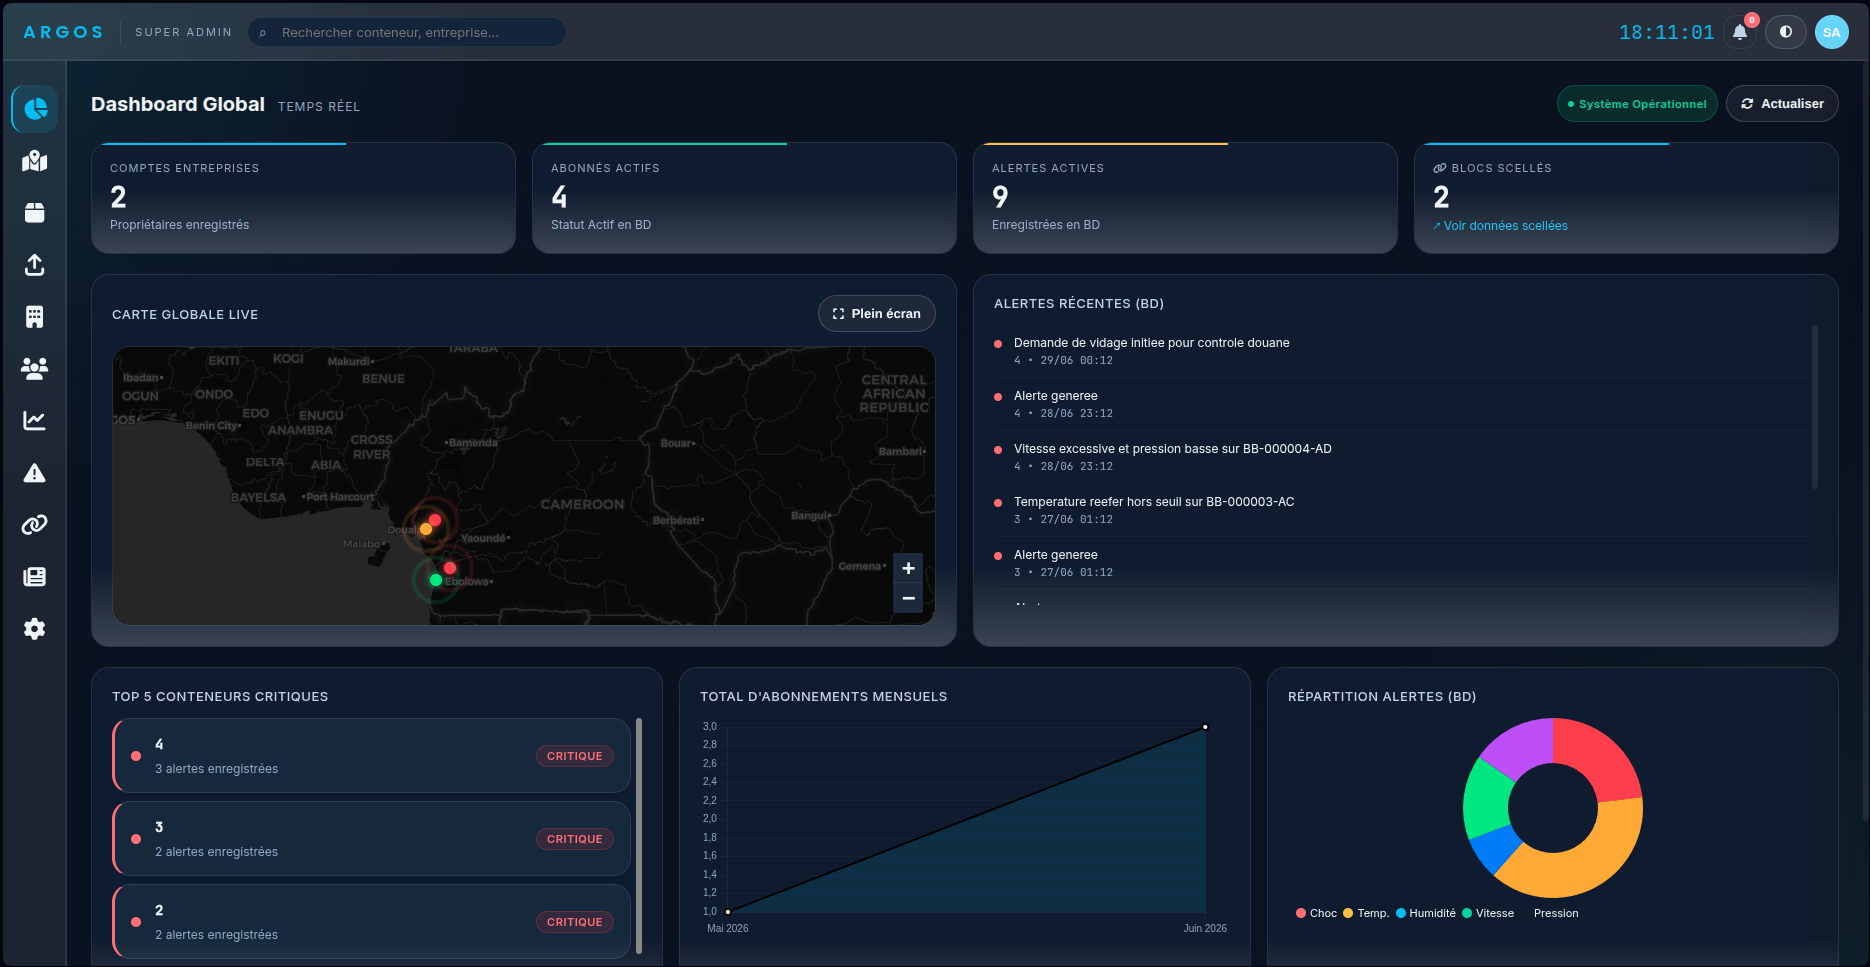
\includegraphics[width=0.66\textwidth]{figures/dash.png}
\vspace{0.5cm} % Petit espace ajouté pour séparer les deux images
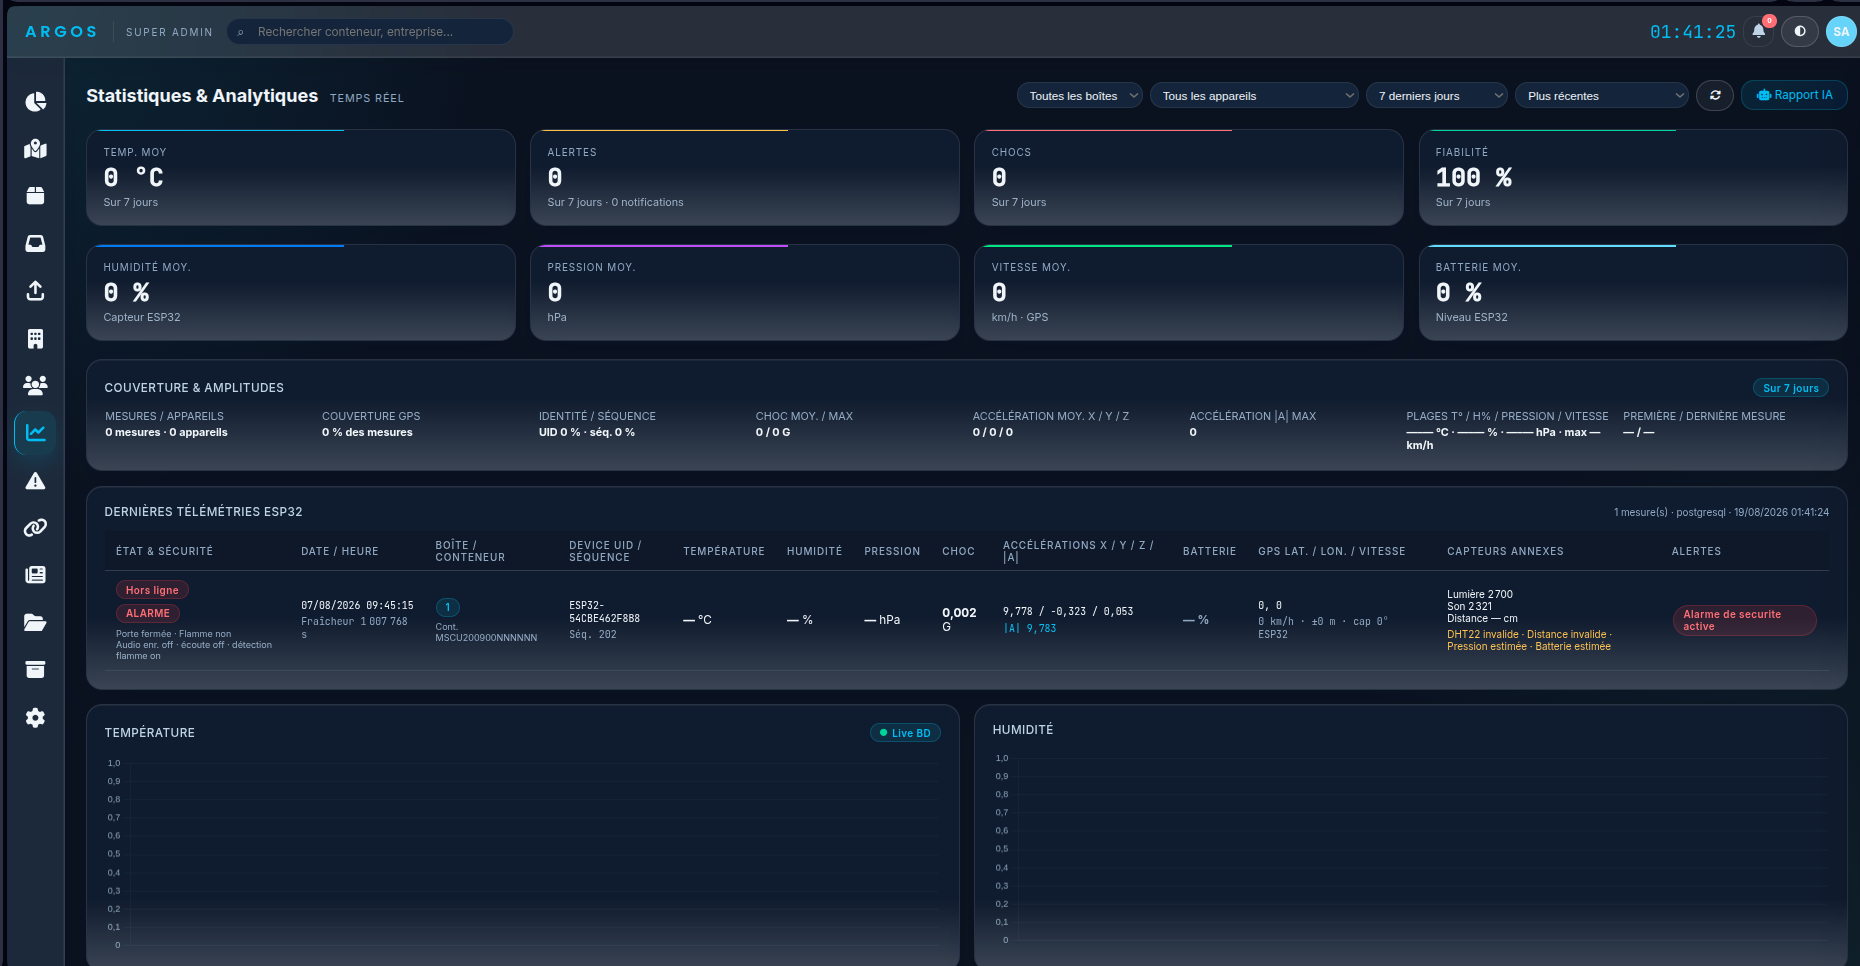
\includegraphics[width=0.66\textwidth]{figures/donnee.png}
\caption{Tableau de bord de supervision ARGOS}
\label{fig-dashboard-argos}
\end{figure}
\tablesourcepromoteurs


\subsection{Validation expérimentale}

\subsubsection{Tests déjà présents}

Les tests logiciels couvrent notamment la validation des coordonnées, les
types de capteurs, les statuts de commande, l'identité signée, le
provisionnement, la résolution QR et la protection des documents. Ils
constituent une validation du contrat logiciel entre le dispositif et le
backend.

\subsubsection{Protocole de mesures sur le prototype physique}

\begin{table}[!htbp]
\centering
\caption{Plan de validation expérimentale du prototype}
\label{tab-validation-prototype}
\begin{tabularx}{\textwidth}{@{}p{3.5cm} X p{3.2cm}@{}}
\tableheadrow \thc{Mesure} & \thc{Méthode proposée} & \thc{Résultat} \\
\midrule
Latence de télémétrie & Mesurer le délai entre l'émission série et la
confirmation du serveur sur 100 messages & Intervalle d'actualisation : 2~s \\
\hline
Taux de livraison & Comparer les séquences émises aux messages persistés,
avec et sans coupure réseau & 900 messages transmis sur 900 (100~\%) \\
\hline
Précision GPS & Comparer plusieurs positions à une référence connue en
extérieur & Précision horizontale : 5~m \\
\hline
Température, humidité et pression & Comparer les capteurs à des instruments de référence
dans plusieurs conditions & 25,45--28,55~\textdegree C ; 64,6--71,4~\% ;
1007,65--1010,35~hPa \\
\hline
Choc et vitesse & Étalonner le MPU-6050, provoquer des accélérations contrôlées
et comparer la vitesse fusionnée à la vitesse GNSS & Choc maximal : 7,35~g ;
vitesse : 54--70~km/h \\
\hline
Autonomie & Calculer puis vérifier la durée avec la batterie réellement
installée & Batterie : 100~\% à 98~\% après 30~min \\
\hline
Réaction à une alerte & Provoquer un dépassement contrôlé et mesurer le délai
jusqu'à la notification & Alerte déclenchée dès le dépassement de 5~g \\
\tablebottomrule
\end{tabularx}
\end{table}
\tablesourcepromoteurs

La réalisation du prototype démontre la continuité technique entre
l'acquisition embarquée, la communication réseau, la validation serveur, la
persistance et la supervision web. Le simulateur permet de tester les mêmes
contrats d'API indépendamment du montage physique. Le protocole expérimental
défini dans ce chapitre assure la traçabilité des performances mesurées lors
de la validation finale.
\\
\\
\\
\\
\\
\\
\\
\\
\\
\\
\\
\\
\\
\\
\\
\\
\subsection{Processus de déploiement}
\begin{figure}[h]
    \centering
    \begin{tikzpicture}[
        node distance=1.8cm,
        auto,
        % Style des boîtes d'étape
        box/.style={
            rectangle,
            rounded corners=4pt,
            draw=black, 
            thick,
            fill=blue!5,
            text width=11cm,
            align=left,
            inner sep=8pt,
            minimum height=1cm
        },
        % Style de la boîte finale
        finalbox/.style={
            rectangle,
            rounded corners=4pt,
            draw=green!60!black, 
            thick,
            fill=green!10,
            text width=11cm,
            align=center,
            inner sep=8pt,
            minimum height=1cm
        },
        % Style des flèches
        arrow/.style={
            thick,
            ->,
            >=stealth
        }
    ]

    % Définition des nœuds (étapes)
    \node[box] (step1) {\textbf{1. Financement \& Incubation} \\ Levée de fonds (prêts bancaires, investisseurs) et accompagnement par l'incubateur de SUP'PTIC.};
    
    \node[box, below of=step1, yshift=-0.5cm] (step2) {\textbf{2. Création \& Certification d'Entreprise} \\ Structuration juridique et certification officielle du projet sous l'entité ARGOS.};
    
    \node[box, below of=step2, yshift=-0.5cm] (step3) {\textbf{3. Agrément International (OMI)} \\ Négociations avec l'Organisation Maritime Internationale pour certifier la conformité, la fiabilité et la déployabilité de la solution.};
    
    \node[box, below of=step3, yshift=-0.5cm] (step4) {\textbf{4. Facilitation Douanière} \\ Enregistrement du dispositif à la douane en tant qu'« équipement de transit » afin de bénéficier d'exonérations fiscales.};
    
    \node[box, below of=step4, yshift=-0.5cm] (step5) {\textbf{5. Déploiement Commercial} \\ Présentation de la solution aux partenaires commerciaux, appuyée par une preuve de concept (PoC) garantissant la véracité des données.};
    
    \node[box, below of=step5, yshift=-0.5cm] (step6) {\textbf{6. Partenariats Assurances} \\ Négociations avec les compagnies d'assurance pour imposer l'installation du dispositif ARGOS sur les conteneurs couverts.};
    
    \node[finalbox, below of=step6, yshift=-0.5cm] (step7) {\textbf{7. Mise sur le Marché \& Opérationnalisation} \\ La solution ARGOS est officiellement déployée et fonctionnelle sur le marché de la logistique.};

    % Tracé des flèches
    \draw[arrow] (step1) -- (step2);
    \draw[arrow] (step2) -- (step3);
    \draw[arrow] (step3) -- (step4);
    \draw[arrow] (step4) -- (step5);
    \draw[arrow] (step5) -- (step6);
    \draw[arrow] (step6) -- (step7);

    \end{tikzpicture}
    \caption{Feuille de route du déploiement de la solution ARGOS}
    \label{fig:deploiement_argos}
\end{figure}